\documentclass[../main.tex]{subfiles}
\begin{document}

\subsection{Setup and Method}
We believe that an alternative implementation of an existing CCA can be evaluated using two metrics. First, whether or not the behavior of the implementation matches (to a reasonable extent) existing implementations of the same CCA. Secondly, the performance costs of the implementation when compared to other implementations. We included two sets of benchmarks to measure this: a behavioral benchmark aimed to verify the "correctness" of different implementations (TCP Cubic should behave similarly no matter where it is implemented, as indicated by metrics such as bitrate/congestion window size over time), and a performance benchmark aimed to measure the CPU overhead of different implementation approaches. A CCA implementation with smaller CPU overhead would logically lead to a higher maximum bandwidth in an ideal, infinite-speed connection where the CPU running the CCA is the bottleneck. \\
Our benchmarks are ran with iperf3 \cite{iperf}. For each trial, we loop through every CCA we are testing and run iperf3 for 15 seconds. At the same time, we run a Python script that loops infinitely and adds 1 to an accumulator at every loop. Once the 15 seconds are up, the script then outputs the final number into a file, a higher number suggesting that the script was able to access more CPU cycles. We ran 20 trials to ensure statistical reliability. Our testing script also included various parameters that can be tuned, including trial duration, reporting intervals, and the metric to be used while generating graphs for the behavioral benchmark. \\
After all the trials, we average the behavioral metric across the trials and plot the average for each CCA through time as the behavioral benchmark. We then plot the CPU performances for each CCA across trials on a boxplot. \\

In order to make sure we are correctly benchmarking the performance impact of CCAs rather than miscellneous confounding factors, we ran the benchmark on an out-of-the-box Debian image on a VM. To ensure the CPU benchmark and the CCA are running on the same CPU, our VM is set up to contain only one core. We also decided to run our benchmarks on various implementations of TCP Cubic due to its wide availability across platforms.

\subsection{Results}

\begin{figure}[t]
    \centering
        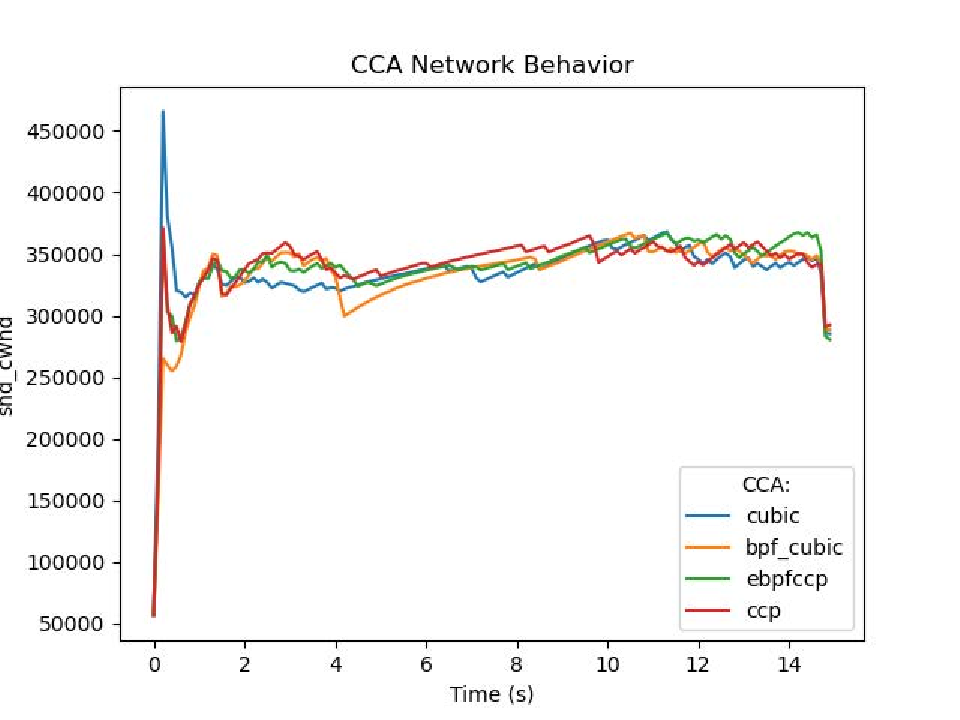
\includegraphics[width=\columnwidth]{img/cca-behavior-cwnd}
        \caption{snd-cwnd behavior of TCP Cubic across different platforms of implementation. Averaged over 20 trials.
        }\label{fig:cca-behavior-cwnd}
    \end{figure}

\begin{figure}[t]
    \centering
        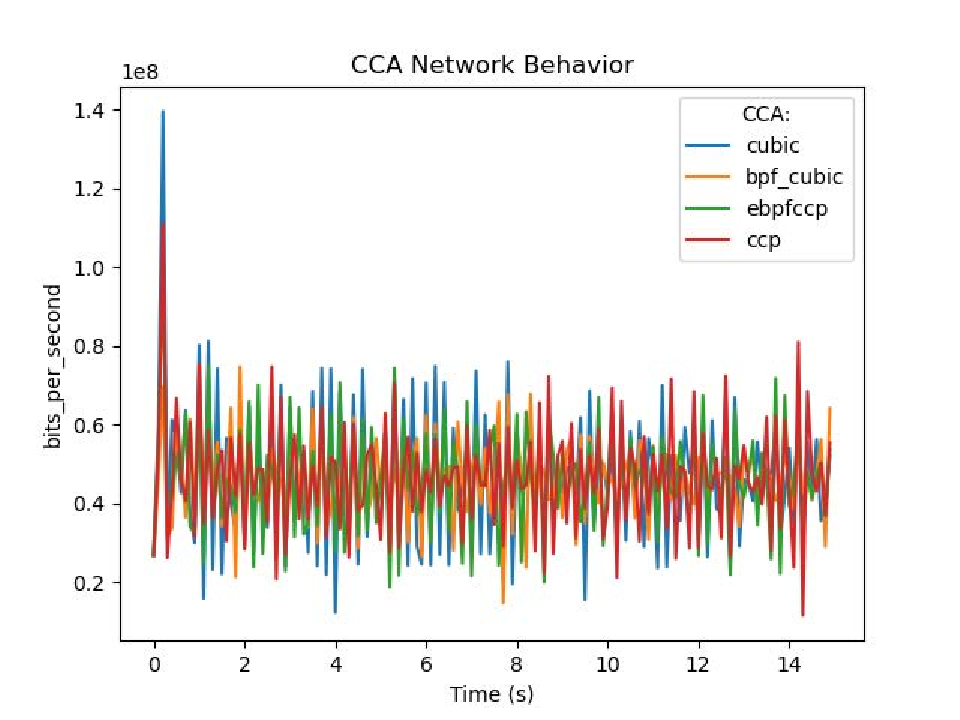
\includegraphics[width=\columnwidth]{img/cca-behavior-bitrate}
        \caption{Bitrate behavior of TCP Cubic across different platforms of implementation. Averaged over 20 trials.
        }\label{fig:cca-behavior-bitrate}
    \end{figure}

\begin{figure}[t]
    \centering
        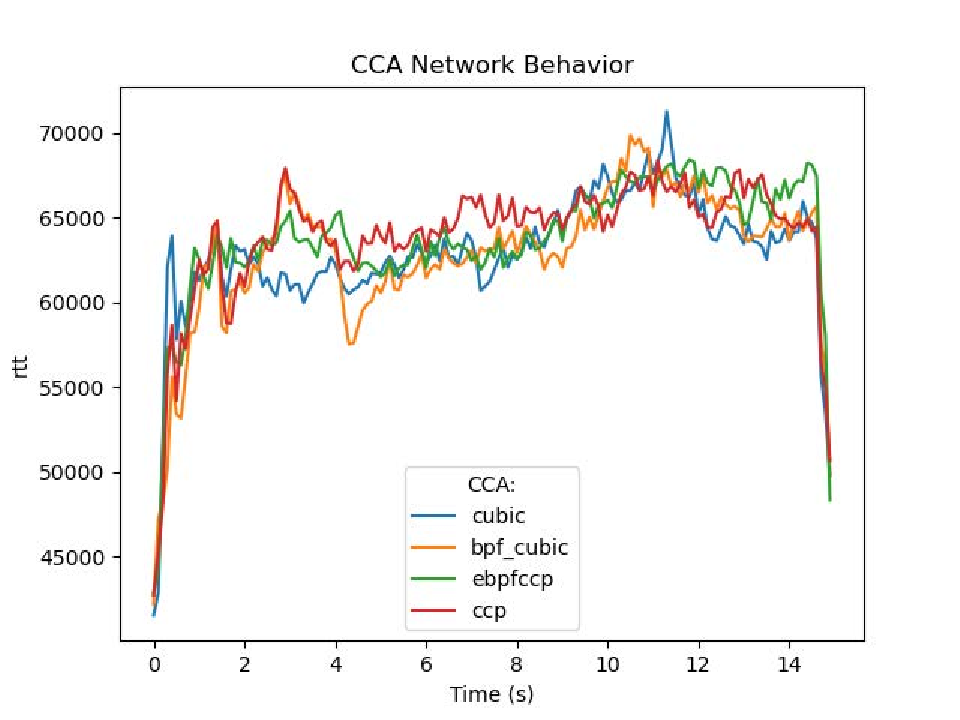
\includegraphics[width=\columnwidth]{img/cca-behavior-rtt}
        \caption{RTT behavior of TCP Cubic across different platforms of implementation. Averaged over 20 trials.
        }\label{fig:cca-behavior-rtt}
    \end{figure}

\begin{figure}[t]
    \centering
        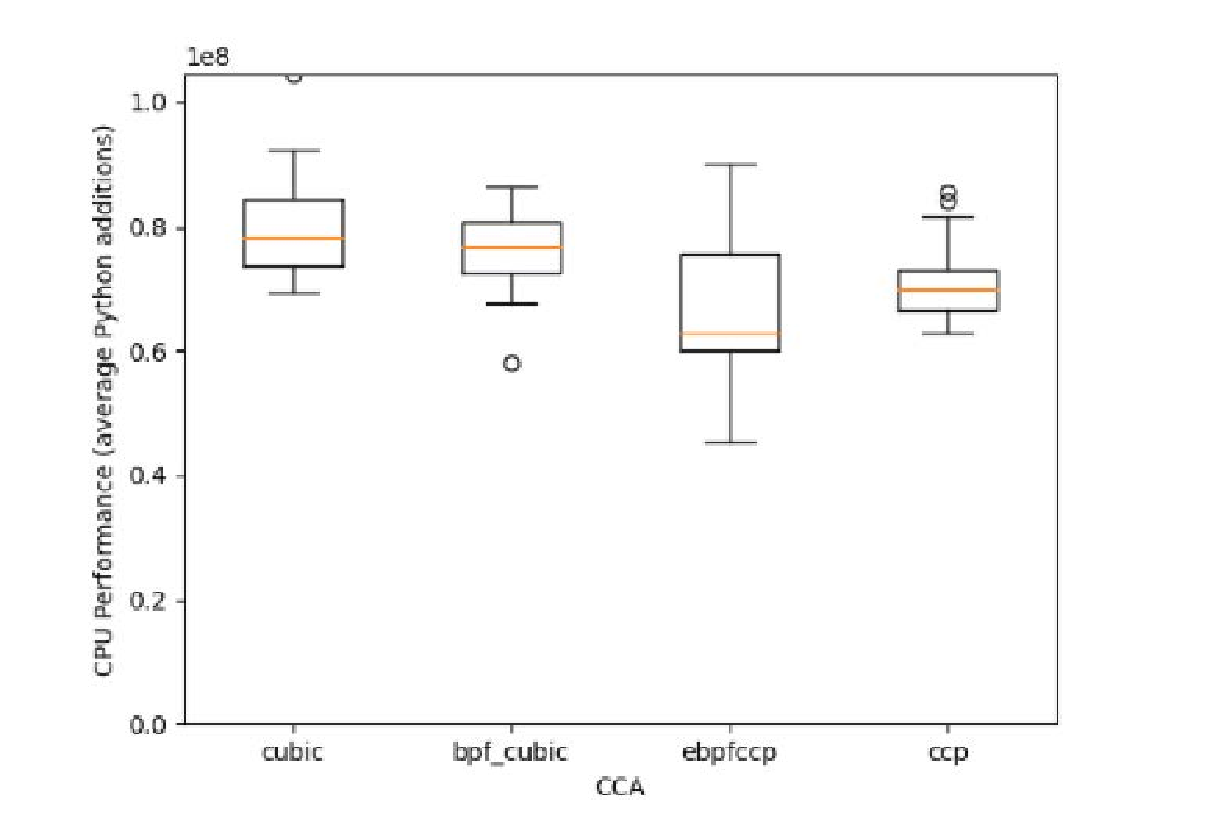
\includegraphics[width=\columnwidth]{img/cca-performance}
        \caption{Standard box plot of TCP Cubic CPU performance across different platforms of implementation. Higher is better. Box extends from 25th to 75th percentile. Whiskers extend to the farthest data point within 1.5 IQR from the box. Data gathered over 20 trials.
        }\label{fig:cca-performance}
    \end{figure}

The results of behavioral benchmarks are shown in Figures~\ref{fig:cca-behavior-cwnd},~\ref{fig:cca-behavior-bitrate}, and~\ref{fig:cca-behavior-rtt}. From the graph, we can see that the behavior of the same Congestion Control Algorithm remains similar across multiple platforms of integration. These results gives us confidence on the correctness of all the implementation platforms involved, and allows us to proceed to performance benchmarking. The results of CPU benchmarks are shown in Figure \ref{fig:cca-performance}. The eBPF implementation of TCP Cubic achieved impressive CPU performance compared to the built-in Linux kernel networking stack implementation. CCP-Cubic from the CCP Project \cite{generic-cong-avoid} combined with the kernel module + netlink CCP datapath achieved slightly lower performance, where its median is at x percent of the full kernel implementation value. Our implementation of eBPFCCP ranked lower on the performance chart, but was still able to achieve y percent of the full kernel implementation value. Due to the relative comparability of CPU performance between the kernel and eBPF implementations of TCP Cubicm, we theorize the gap between eBPFCCP and kernel module CCP was due to our choice of using unix pipes rather than netlink as a channel for communicating between the eBPFCCP and the user space program. \\
From these results, we can conclude that eBPF is a viable platform for the development CCAs. The negligible performance overhead when compared to the kernel native implementation is impressive, and suggests that eBPF-CCAs can possibly also be used as a long-term deployment option outside of research and development stages. With regards to CCP, while the performance overhead of eBPFCCP is non-negligible, it should be noted that the benchmark is performed on a single core VM. In a real-world scenario, the performance overhead of eBPFCCP is likely to be negligible for all but the most performance-sensitive industry networking applications. The safety guarantees provided by eBPFCCP would provide a good intermediate step for users to adopt and experiment with a new CCA before it is natively implemented either directly into the kernel or as an eBPF program. 
\end{document}
